% ============================================================================
% ICME 2027 submission — Plan B (repositioned 2026-11-06)
% ----------------------------------------------------------------------------
% Template basis: official ICME 2026 author kit (downloaded 2026-11-06 from
%   2026.ieeeicme.org/.../IEEE-Conference-Template-ICME-2026.zip)
%   -> \documentclass[conference]{IEEEtran}, \author{Anonymous ICME submission},
%      \bibliographystyle{IEEEbib}
%
% Page budget (D1=A, frozen by Lead): **6 pages INCLUDING all text, figures and
%   references** (2024/2025/2026 ICME official wording identical; ICME 2027 CFP
%   not yet published -> marked "per ICME 2024-2026 official page limit").
%
% Plan B positioning (Lead decision 2026-11-06, after the unified-recipe fair
%   ablation): benchmark + diagnostic study + controlled-intervention protocol.
%   The regularizer section is a controlled intervention, NOT a proposed method;
%   no performance claim over identity/hard controls is made.
% ============================================================================
\documentclass[conference]{IEEEtran}
% \IEEEoverridecommandlockouts   % only needed for a funding footnote; unused in the double-blind copy
\usepackage{cite}
\usepackage{amsmath,amssymb,amsfonts}
\usepackage{graphicx}
\usepackage{textcomp}
\usepackage{xcolor}
\usepackage{booktabs}
\usepackage{array}
\usepackage{multirow}
\usepackage{pifont}
\usepackage[hidelinks]{hyperref}

% ---------------------------------------------------------------------------
% Project macros — names mirror cvpr2027/preamble.tex (keep identical so that
% sections migrated from the frozen base compile unchanged).
% ---------------------------------------------------------------------------
\newcommand{\Om}{\Omega}
\newcommand{\dOm}{\partial\Omega}
\newcommand{\T}{\mathbf{T}}
\newcommand{\I}{\mathbf{I}}
\newcommand{\R}{\mathbf{R}}
\newcommand{\That}{\widehat{\mathbf{T}}}
\newcommand{\Rhat}{\widehat{\mathbf{R}}}
\newcommand{\quiet}{\mathcal{L}_{\mathrm{quiet}}}
\newcommand{\reg}{\mathcal{L}_{\Om}}
\newcommand{\dBA}{\,\mathrm{dB}}
\newcommand{\PSNOm}{\mathrm{PSNR}_{\Om}}
\newcommand{\red}[1]{{\color{red}#1}}
\newcommand{\todo}[1]{{\color{red}#1}}

% ---------------------------------------------------------------------------
% Figure path: local fig/ (staged by planB_build.ps1 from the frozen base; the
% output/ tree is not writable from this shell), then the frozen fig dir.
% ---------------------------------------------------------------------------
\graphicspath{{fig/}{../cvpr2027/fig/}}

\title{What Filmed Glass Does to Single-Image Reflection Removal:\\
A Development Benchmark and a Diagnostic Study}

\author{Anonymous ICME submission}

\begin{document}
\maketitle

% ============================================================================
% sec0_abstract.tex — Abstract + keywords (Plan B, 2026-11-06)
% Constraints: 100-150 words; no math/symbols; only Plan B citable numbers;
% "development benchmark/panel"; no method claim.
% ============================================================================
\begin{abstract}
Single-image reflection removal (SIRR) assumes a friendly photometric regime: a
bright reflection layered over a well-exposed scene. Automotive window film breaks
this premise: the film sits on the scene side, so transmitted light is scattered and
dyed while the reflection comes off the bare surface. Even a recent lightweight
method fine-tuned in-domain with its official recipe remains 2.2 dB behind our uniform-recipe baseline (22.38\,dB). We present a hand-annotated 15-scene real-pair development
benchmark for filmed glass and use it to measure two failure axes: transmission
loses high-frequency content while reflection stays sharp (an empirical layer
asymmetry), and the global photometric level is not identifiable from a single
frame. We then report a pre-registered, unified-recipe control experiment that
bounds what training-time regularization can achieve on this benchmark, and
quantify the run-level reproducibility that this control must exceed.
\end{abstract}

\begin{IEEEkeywords}
single-image reflection removal, filmed glass, real-pair benchmark, diagnostic study, evaluation protocol, run-level reproducibility
\end{IEEEkeywords}

% ============================================================================
% sec1_intro.tex — Introduction (Plan B version, 2026-11-06)
% Fig.1 = 0.58 width figure*; contributions C1-C4 per Lead execution order.
% ============================================================================
\section{Introduction}
\label{sec:intro}

\begin{figure*}[t]
\centering
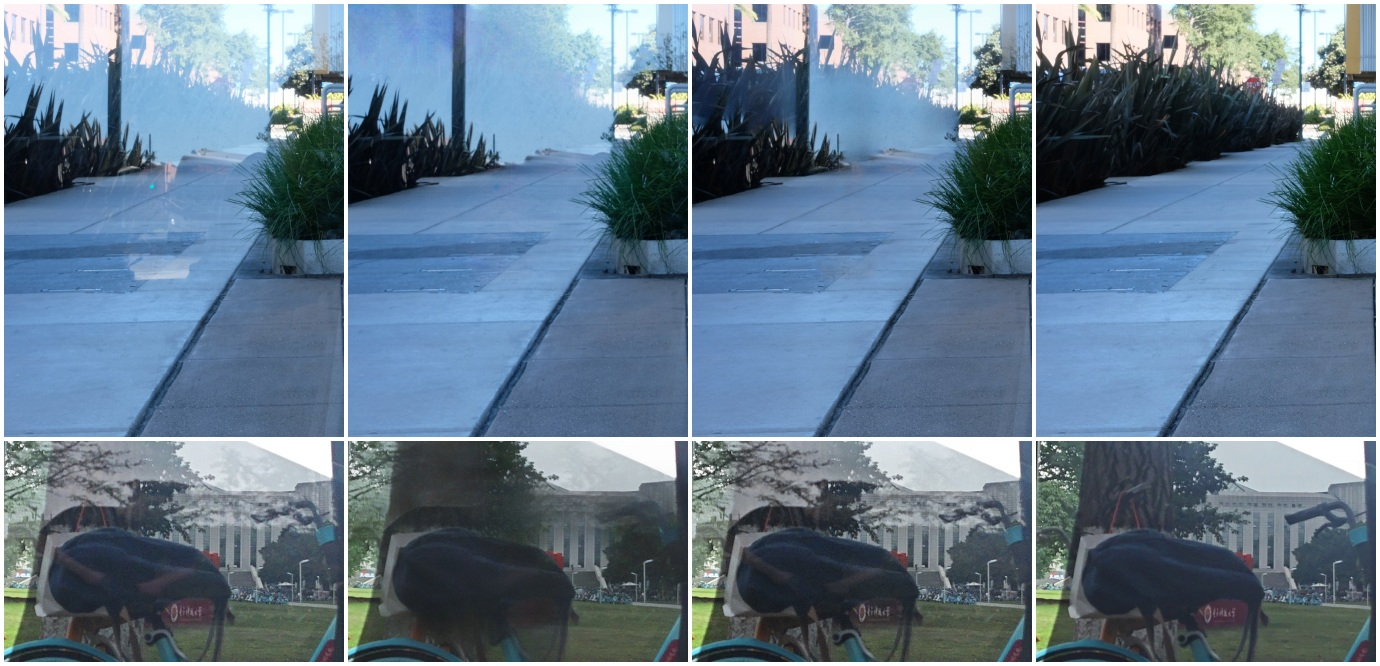
\includegraphics[width=0.58\textwidth]{fig/teaser_2rows.jpg}
\caption{\textbf{Same model, two kinds of glass.} Top: on Real20 a state-of-the-art
method removes the reflection almost completely while a light-weight model removes only
part of it. Bottom: on a filmed-glass pair the same method darkens the frame and strips
transmitted detail instead of removing the reflection, and the light-weight model
changes almost nothing. The difference is not the network but the imaging: the film sits
on the scene side, so transmitted light is scattered and dyed while the reflection comes
off the bare glass surface.}
\label{fig:teaser}
\end{figure*}

Single-image reflection removal (SIRR) addresses a situation any camera user has met:
a photograph through a pane of glass, in which the scene behind the camera is
superimposed on the scene in front of it. The setting---car windows, shop facades,
museum cases, aquaria---is ubiquitous; SIRR is a standing task.
The dominant recipe is data-driven: paired corpora, a network
regressing the transmitted layer, and a loss on deviation from the clean
reference. Successive generations---classical layer priors, cascaded and recurrent
designs, reversible and dual-stream architectures, and recently diffusion
priors~\cite{wan2017benchmarking,wan2022crrn,li2020ibcln,wen2019errnet,zhao2025rdnet,hu2024dsit,hu2023dsrnet,hong2024ldiffer,promptrr2024,li2026gensirr,hu2026dai,xu2026fumo}---have
advanced the state of the art on benchmarks such as
Real20~\cite{zhang2018perceptual} and SIR$^2$~\cite{wan2017benchmarking}.

What these recipes share is an assumption about the \emph{glass}. In deployment the
glass is rarely bare: automotive and architectural glazing is almost always
\emph{filmed}, for heat rejection, privacy and UV protection, and a dark film changes
the imaging. The film is laminated on the scene side, so the light we want travels
through it---scattered, absorbed and dyed---while the light to discard comes off the bare
surface facing the camera. The observed image is a sharp
reflection over a soft, desaturated transmission: the layers separate in band and
chroma, not in level. Methods trained on ordinary glass do not expect this, and
empirically do not survive it (Fig.~\ref{fig:teaser}).

SIRR has been attacked with stronger backbones, reversible connections, reflection-rate
estimates and generative priors. What these efforts
share is where they are measured: on benchmarks whose reflections are dense and cover
most of the frame, so a whole-image average already describes the failure. Three things
are consequently missing: to our knowledge, no real paired dataset shot through filmed
glass has been released, so the regime cannot be measured; no analysis of \emph{where}
a method fails, because one average cannot separate regions where removal is necessary
from those where it is harmful; and, consequently, training losses inherited from
dense-reflection settings.

This paper takes the opposite order. We first ask what filmed glass does to the two
layers and measure: the transmitted layer loses high-frequency content while the
reflection stays sharp, so detail and discardable content separate in band rather than
brightness (Sec.~\ref{sec:imaging}). We then
ask \emph{where} current methods fail: the reflection is weakest inside the region
blocked by the photographer, where almost nothing needs to change, and strongest in the
annulus around it, which is large and where each of the baselines we tested is at its
worst; because it borders a nearly correct region, its residual is read by the eye as a
\emph{boundary} (Sec.~\ref{sec:diagnosis}). Finally we ask what training signal
achieves. A region-relative error is the load-bearing term in development ablations; an
area-matched random-region control indicates that its value comes from normalising by the
local reflection amplitude rather than from the region's identity, so we reduce it to a
mask-free per-pixel regularizer (Sec.~\ref{sec:method}) and test it as a controlled
intervention against identity, magnitude-matched, hard-threshold and shuffled controls
under one training recipe (Sec.~\ref{sec:exp}). We close by stating what the development
panel can and cannot support (Sec.~\ref{sec:discussion}).

\paragraph{Contributions.}
\begin{itemize}
\item \textbf{Data.} A hand-annotated 15-scene real-pair development benchmark for filmed
glass, with training pairs from sessions with locked exposure and white balance and an
explicit quantification of the capture defects (Secs.~\ref{sec:imaging}--\ref{sec:panel}).
\item \textbf{Diagnosis.} A diagnosis organized around two failure axes---transmission
loses high-frequency content while reflection stays sharp (an empirical layer
asymmetry), and the global photometric level is not identifiable from a single
frame---with current methods failing in the annulus around the occluder region
structurally rather than photometrically (Sec.~\ref{sec:diagnosis}).
\item \textbf{Protocol.} A pre-registered, unified-recipe control protocol: a mask-free
change-aware regularizer tested against identity, magnitude-matched, hard-threshold and
shuffled controls over three seeds, bounding what training-time regularization achieves
on this benchmark while disclosing run-level reproducibility (Sec.~\ref{sec:exp}).
\item \textbf{Boundary.} An honest statement of where claims stop: occluder-region
specificity is withdrawn, no public-benchmark state-of-the-art claim is made, the panel
is a development panel with a stated minimum detectable effect, and several negative
results are reported (Sec.~\ref{sec:discussion}).
\end{itemize}

\paragraph{Organisation.} Sec.~\ref{sec:related} reviews related work;
Secs.~\ref{sec:imaging}--\ref{sec:method} present the study;
Secs.~\ref{sec:exp}--\ref{sec:discussion} report experiments and limitations.

% ============================================================================
% sec2_related.tex — Related Work (Plan B version, 2026-11-06)
% ============================================================================
\section{Related Work}
\label{sec:related}

\paragraph{Single-image reflection removal and the average metric.}
SIRR has a long line of work. Classical methods exploit gradient sparsity and layer
priors~\cite{wan2017benchmarking,wan2022crrn}; deep methods regress the transmitted
layer: ERRNet aligns misaligned pairs~\cite{wen2019errnet},
IBCLN cascades refinement~\cite{li2020ibcln}, DSRNet models component
synergy~\cite{hu2023dsrnet}, dual-stream transformers add cross-layer
interaction~\cite{hu2024dsit}, RDNet uses a reversible encoder with a transmission-rate
condition~\cite{zhao2025rdnet}, and RRW revisits real-world data
collection~\cite{zhu2024rrw}. Generative routes---language-conditioned, prompt-based and
prior-modulated diffusion, and latent-space rectification---recently pushed
synthetic-benchmark quality
further~\cite{hong2024ldiffer,promptrr2024,li2026gensirr,hu2026dai,xu2026fumo,chen2026gfrrn}.
Nearly all are evaluated by a whole-image average on Real20~\cite{zhang2018perceptual},
SIR$^2$~\cite{wan2017benchmarking}, RRW~\cite{zhu2024rrw} or their own splits, where
reflection is dense; an average then already describes the failure, and spatially
compact failures---our topic---are diluted rather than measured.

\paragraph{Real-pair protocols and benchmarks.}
Real-pair supervision needs the same scene with and without reflection.
Three routes exist: removing the glass (refraction misalignment and illumination
change), a polariser or flash (hardware a single RGB frame
lacks~\cite{lei2020polarized}), or dark cloth over the camera side (misalignment traded
for exposure and white-balance drift). The black-cloth route underlies recent corpora
and challenges~\cite{zhu2024rrw,openrr2025,cai2026ntire}. All three assume the cover is
complete, and to our knowledge none records where the reflection was suppressed. Our
data keeps and annotates the partial case---normal when shooting through a car
window---and quantifies its two defects. Region-conditioned methods such as
LANet~\cite{lanet2021} learn where reflection exists, whereas our occluder region is
where reflection is weakest.

\paragraph{Loss weighting and identity-regulariser precedents.}
Using a difficulty or region measure to weight a loss is standard elsewhere: focal loss
down-weights easy examples~\cite{lin2017focal}, GHM re-balances by gradient
density~\cite{li2019ghm}, learning-to-reweight adapts sample weights~\cite{ren2018reweight},
uncertainty weighting learns task
weights~\cite{kendall2018uncertainty}, adaptive robust losses reshape the penalty by
residual scale~\cite{barron2019robust}, and CycleGAN's identity loss penalises deviation
from an input reference~\cite{zhu2017cyclegan}. Our regularizer is closest to the last
two but differs: its weight is neither a free parameter nor a learned function nor a
schedule---it is computed from the pair's own residual, acts on the
output-minus-input difference, and vanishes where no change is needed, so the baseline
is a strict special case. Sec.~\ref{sec:exp} tests it against identity,
magnitude-matched, hard-threshold and shuffled controls under one recipe.

% ============================================================================
% sec3_imaging.tex — Filmed glass: imaging, capture and panel (§3, W1 rev2)
% Target: ~545 words (Lead: must fit the 5.12 p body budget; trim in-section).
% Numbers only from plan 附B (B01-B14, B06-B07); Table I lives in supplementary S2.
% ============================================================================
\section{Filmed Glass: Imaging, Capture and Panel}
\label{sec:imaging}

\subsection{What the film does to the two layers}
\label{sec:film}

For a sensor measurement through a filmed pane,
$I(x)=\tau\,T(x)+\rho\,R(x)$, where $\tau$ is the film-attenuated transmission, $\rho$
the reflection coefficient, $T$ the scene and $R$ the reflected environment. Standard
SIRR implicitly assumes that $\rho R$ is bright and $\tau T$ well exposed; window film
challenges both. Since the film is laminated on the scene side and the camera on the
bare side, transmitted light passes \emph{through} the film bulk and is scattered,
absorbed and dyed, whereas the reflection of the behind-camera environment comes off the
bare \emph{surface} and enters no film. The predicted asymmetry in sharpness and chroma
is what we observe. With $\mathrm{sharp}(X)=\mathbb{E}|\mathrm{HP}(X)|/\mathbb{E}|X|$
(HP: unit-variance high-pass) averaged per dataset, filmed glass has
$\mathrm{sharp}(T)=0.027$ against $0.041$--$0.062$ on SIR$^2$-Wild, SIR$^2$-Obj and
Real20, i.e.\ its transmission is about $2.3\times$ softer; the
reflection-to-transmission sharpness ratio is $6.76$ against $2.51$--$3.32$ ($2.0\times$
sharper relative to the layer beneath); and the transmission chroma is $0.219$ against
$0.322$--$0.393$. Mean brightness, mean reflection magnitude and the high-frequency
\emph{fraction} of the reflection are, by contrast, indistinguishable from Real20 when
measured identically on the four datasets: the asymmetry, not brightness, separates the
regimes (full table in the supplementary material).

The film also changes \emph{which} pixels are damaged. Sorting scene pixels by
ground-truth luminance, the reflection magnitude $|I-T|$ is $23.1$ gray levels in the
darkest quartile against $14.1$ in the brightest (the four quartiles give $23.1$, $25.7$,
$17.7$, $14.1$): the two layers are degraded \emph{in the same places}, the opposite of
the usual SIRR setting, where a bright reflection sits on a well-exposed scene.

\subsection{Capture protocol and the ground-truth hazard}
\label{sec:protocol}

All scenes are shot on a phone through an automotive window film, handheld, with
exposure and white balance locked. For each scene we record a short clip with reflection
and then cover the glass with dark cloth to obtain $T$: one $T$ per scene, many $I$;
inputs are extracted at 30\,fps, cropped to the glass area, and a pair is kept only if
the phase-correlation shift is $\le2$\,px and the per-channel gain deviation
$\le0.15$. Covering the glass is not neutral, and on a pool of $82$ confirmed pairs we
report three separate measurements rather than a single causal chain: the transmission
reference is $3.7\%$ darker inside the hand-annotated occluder region than outside
($T_{\mathrm{in}}/T_{\mathrm{out}}=0.963$); the reflected content inside the region is
lower than outside by $16.8\%$ ($r_{\mathrm{in}}/r_{\mathrm{out}}=0.832$); and the
input-to-target ratio is $I/T|_{\mathrm{in}}\approx0.887$ against $1.045$ outside. The
reflection contributes a median $4.5\%$ over the target outside the region ($33\%$ in the
strongest decile). Exposure must be locked: with auto-exposure active we measured
$\mathrm{median}(I/T)=0.99$ and a residual layer correlated with image brightness at
$r=0.32$; after locking, $r=-0.01$. Because $T$ is a separate frame, alignment is a
second hazard: on one batch $88.7\%$ of the pairs were shifted by more than $3$\,px
(median $8.2$\,px). Per-pair translation alignment is a single-seed screening result on
this pool (aligned pool $21.43$\,dB; discarding the $99$ worst pairs gives $+0.80$\,dB)
and is not used for any main-table claim.

\subsection{Development panel and metrics}
\label{sec:panel}

The panel contains 15 scenes ($1280{\times}832$) shot through the filmed pane. For every
scene we hand-annotated the occluder region $\Om$ once (median $4.6\%$ of the image,
range $2.9$--$9.2\%$, under a fixed intensity rule); it marks where the reflection path
was blocked, and it is an annotation, not a physical ground truth. We report PSNR, SSIM,
HF-PSNR, gradient cosine, the Laplacian-variance ratio
$\mathrm{LapVar}(\That)/\mathrm{LapVar}(T)$ and region-restricted PSNR inside/outside
$\Om$, plus the residual-reflection coefficient
$\beta=\langle T-\That,\,I-T\rangle/\lVert I-T\rVert^{2}$ ($-1$: nothing removed, $0$:
perfect) and the per-image gain
$\alpha=\mathrm{median}_i(\overline{\That_i}/\overline{T_i})$. With $n=15$ scenes the
minimum detectable effect of the paired panel is $\approx0.26$\,dB, and the floor for
brightness-only effects is $1.19$--$1.31$\,dB. The panel was used while developing the
annotation protocol and the pilot models, so we call it a \emph{development panel} and
treat its numbers as development-set evidence rather than confirmation.

% ============================================================================
% sec4_diagnosis.tex — Where current methods fail (§4, W1 rev2; trimmed in-section)
% Target: ~570 words + Fig.2 (single column). Numbers only from plan 附B (B15-B24).
% ============================================================================
\section{Where Current Methods Fail on Filmed Glass}
\label{sec:diagnosis}

\begin{figure}[t]
\centering
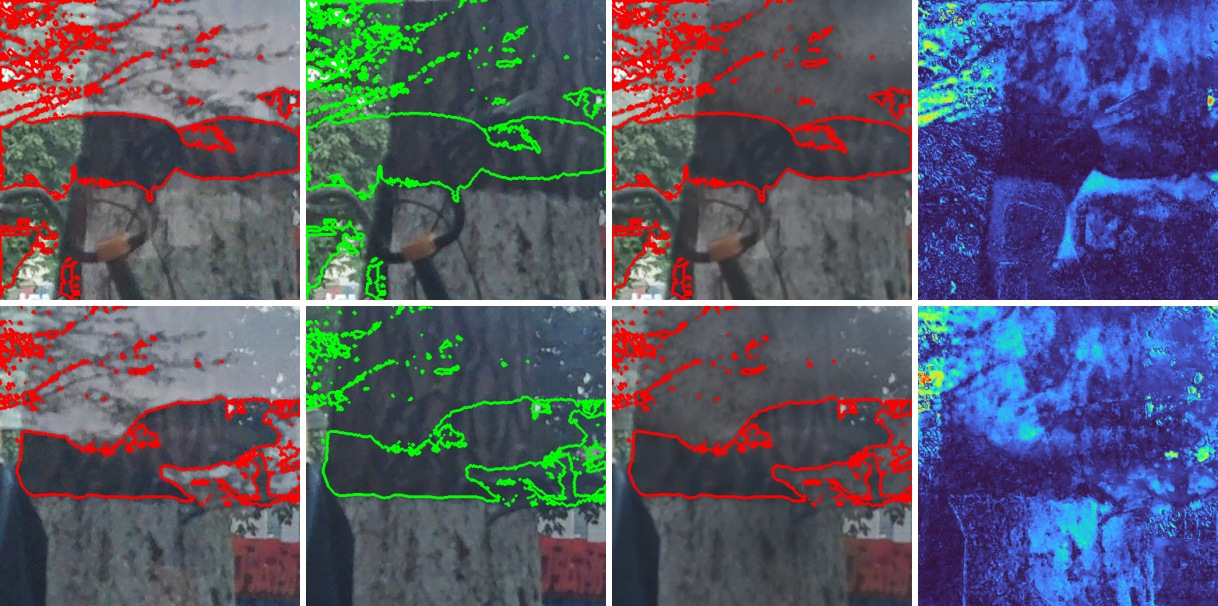
\includegraphics[width=\columnwidth]{fig/qual_omega.jpg}
\caption{\textbf{Where the damage happens.} Two development-panel scenes (rows):
input, ground truth, prediction and per-image-normalised absolute error. Contours mark
the hand-annotated occluder region; the error lights up along it rather than inside the
reflected content.}
\label{fig:qual}
\end{figure}

\subsection{The occluder region needs almost no change; its neighbourhood does}
\label{sec:axis1}

Partitioning each development-panel frame into the hand-annotated occluder region $\Om$,
a $15$\,px annulus around it and the far field gives three very different bands. Inside
$\Om$ the mean reflection magnitude $\mathbb{E}|I-T|$ is only $10.3$ gray levels, and
identity scores $24.52$\,dB, higher than any method in our baseline comparison: almost
nothing needs to change there. The annulus covers $44.4\%$ of the frame and its
$\mathbb{E}|I-T|$ is $44.4$ gray levels, $4.3\times$ that inside $\Om$ and $2.6\times$
that of the far field ($16.8$); identity scores $13.76$\,dB there. The far field lies
in between ($19.52$ identity). The aggregate signature: each of the baselines we tested scores below
identity inside $\Om$ ($\Om$-restricted PSNR $20.89$--$23.55$\,dB against $24.52$, i.e.\
all $\Delta_\Om<0$), and each is at its absolute worst in the annulus ($19.4$--$19.8$\,dB
versus $23.5$ far away). The consequence is perceptual: the annulus abuts an almost correct region, so its
residual is read as a \emph{boundary}; repairing it needs extrapolation from elsewhere in
the frame along semantic continuations rather than more reflection removal.

\subsection{The damage is structural, not photometric}
\label{sec:structural}

A photometric explanation would predict that models merely mis-scale $\Om$; they do not.
Restricting to $\Om$ and allowing a per-image affine correction before scoring, the
structure retained relative to ground truth is $1.14$ for identity, only $0.50$ for the
fine-tuned baseline and $0.65$ with the regularizer (development measurements;
affine-corrected MAE $10.51$, $12.82$, $11.70$ gray levels). We can also bound any content-agnostic method: a Gaussian smoothing
of the input is the best one can do without knowing the content. On the weakly reflected
$59\%$ of $\Om$ that ceiling is $29.50$\,dB against identity's $31.45$ and the
regularizer's $27.18$; on the strongly reflected $7\%$ it is $15.24$\,dB against $14.46$
and $13.48$. None of the models we trained beats a plain blur in either regime. The
remaining photometric head-room is per-image: a per-image affine oracle recovers
$0.15$--$0.26$\,dB whereas a shared leave-one-scene-out affine recovers $0.07$\,dB
(details in the supplementary material).

\subsection{Reflection and scene share the frequency band}
\label{sec:band}

$34.5\%$ of the reflection energy lies above a $\sigma{=}8$ low-pass, so it is not a veil
that can be filtered away. Replacing the low frequencies of a model output by the model's
own and the high frequencies by those of the \emph{input},
$\That'=\mathrm{LP}_\sigma(\That)+(I-\mathrm{LP}_\sigma(I))$, restores structure inside
$\Om$ but \emph{lowers} PSNR: from $22.26$ to $22.04$ and $21.66$\,dB at $\sigma{=}2,4$
(regularized model), and from $23.73$ to $23.39$ and $22.97$\,dB for a $50{:}50$
mixture. The band carrying the missing structure also carries the reflection.

\subsection{The load-bearing term is not about the region}
\label{sec:axis3}

Our objective contains a region-relative error inside $\Om$,
\begin{equation}
\reg=\lambda_{\Om}\,\mathbb{E}_{\Om}\!\left[\frac{|T-\That|}{\mathbb{E}_{\Om}|T-I|}\right],
\label{eq:lom}
\end{equation}
Removing it is catastrophic in a single-seed, pre-unified development ablation: the
panel score falls from $22.49$ to $18.33$\,dB, below identity's $18.44$\,dB (these are
historical numbers, not results of the unified protocol). Its power, however, is not the annotation. Replacing the hand mask by an
equal-area random disk, three seeds on a separate $82$-pair pool, gives $19.90\pm0.16$\,dB
against $19.41\pm0.54$ for the annotated region and $17.76\pm0.16$ for no region:
real-minus-random is $-0.49$\,dB (positive on one of three seeds). A whole-image relative
error without any region reaches $20.05$\,dB and a fixed per-pair disk $20.25\pm0.29$\,dB.
What matters is thus \emph{that a compact region is supervised with a relative
normalization}, not that it is the occluder region; a per-pixel version needs no mask,
which we test as a controlled intervention (Sec.~\ref{sec:method}).

% ============================================================================
% sec5_method.tex — The change-aware regularizer as a controlled intervention
% (Plan B, 2026-11-06: compressed to <=0.15 p; keeps the definition and the
% lambda/tau values; no performance claim, no "our method" wording.)
% ============================================================================
\section{A Mask-Free Regularizer as a Controlled Intervention}
\label{sec:method}

We treat the regularizer as a controlled intervention, not as a proposed method.
The needed-change statistic and the change-aware weight are computed from the
training pair only, and the intervention is evaluated on the output:
\begin{equation}
\begin{aligned}
n(x) &= \tfrac{1}{3}\textstyle\sum_{c}\bigl|I_c(x)-T_c(x)\bigr|, \\
w(x) &= \bigl(1-n(x)/\tau\bigr)_{+},\qquad \tau=0.05, \\
\quiet &= \lambda\,\mathbb{E}\bigl[w(x)\,\bigl|\That(x)-I(x)\bigr|\bigr],\qquad \lambda=1,
\end{aligned}
\label{eq:quiet}
\end{equation}
so a pixel that needs no change is held in place. The weight uses no annotation,
the term adds no parameters and no inference cost, and $w\equiv0$ reduces it to the
baseline. Sec.~\ref{sec:exp} tests it against identity, magnitude-matched,
hard-threshold and shuffled controls under one training recipe.

% NOTE (Plan B): the old "Why this shape" and "Training configuration" subsections
% were removed. The training configuration now lives in the supplementary material
% (S3), together with the arm definitions and the full control table.

% ============================================================================
% sec6_experiments.tex — Experiments (Plan B, 2026-11-06)
% Unified-recipe control experiment + run-level reproducibility + LightRR
% motivation + frozen held-out protocol + negative results.
% All numbers are from the Lead's final unified-script table (15-scene panel,
% hand-annotated Omega, uint8 evaluation; three seeds 101/202/303).
% ============================================================================
\section{Experiments}
\label{sec:exp}

\subsection{Protocol and baselines}
\label{sec:setup}
All scores below are on the 15-scene development panel, produced by a frozen
uint8 evaluation script. Trained arms use seeds $101$, $202$ and $303$; we
report the mean and standard deviation over scenes, and differences are
scene-level paired means with $95\%$ confidence intervals over the 15 scenes.
The fine-tuned baseline is a strongly fine-tuned RDNet~\cite{zhao2025rdnet}
(frozen FocalNet backbone, $65.95$M trainable parameters, $6000$ iterations,
$30/40/30$ real/synthetic/public mixture; supplementary material S3). Zero-shot
public methods range from $18.12$\,dB (IBCLN~\cite{li2020ibcln}) to
$20.50$\,dB (Zhu et al.~\cite{zhu2024rrw}), while a trivial identity
predictor scores $18.44$\,dB and the strongly fine-tuned baseline scores
$22.38\pm0.23$\,dB. We compare public methods zero-shot only and make no
public-benchmark state-of-the-art claim.

\subsection{A unified-recipe control experiment}
\label{sec:control}
To ask what a training-time regularizer can achieve on this benchmark, the
regularizer and four controls share one recipe---identical data mixture,
schedule, seeds and evaluation---so only the extra term differs. The arms are:
\emph{base} (no extra term); \emph{identity} (a plain identity penalty
$\lambda\|\That-I\|_1$ with $\lambda=0.409$); \emph{identity-m} (the same with
$\lambda=0.085$, magnitude-matched to the change-aware weight); \emph{hard}
(the change-aware statistic thresholded at $\tau=0.05$); \emph{shuffled} (the
change-aware weights permuted across pixels); and \emph{full} ($\quiet$ with
$\lambda=1$, $\tau=0.05$). Table~\ref{tab:control} reports the result.

\begin{table}[t]
\centering
\footnotesize
\caption{Unified-recipe control experiment (development panel, $15$ scenes,
three seeds). PSNR is the mean over scenes; $\Delta$ is the scene-level paired
mean against \emph{full} with its $95\%$ CI. All regularized arms sit within
$0.44$\,dB of base.}
\label{tab:control}
\begin{tabular}{lcc}
\toprule
arm & PSNR (dB) & $\Delta$ vs.\ full (dB) \\
\midrule
base (no regularizer)        & $22.38\pm0.23$ & $+0.19\,[+0.05,+0.33]$ \\
identity ($\lambda{=}.409$)  & $22.49\pm0.34$ & $+0.079\,[+0.021,+0.137]$ \\
identity-m ($\lambda{=}.085$) & $22.59\pm0.21$ & $-0.014\,[-0.215,+0.186]$ \\
hard ($\tau{=}.05$)          & $22.82\pm0.36$ & $-0.246\,[-0.355,-0.138]$ \\
shuffled weight              & $22.36\pm0.39$ & $+0.209\,[+0.033,+0.386]$ \\
\textbf{full ($\lambda{=}1$, $\tau{=}.05$)} & $\mathbf{22.57\pm0.00}$ & --- \\
\bottomrule
\end{tabular}
\end{table}

The regularized arms span $22.36$--$22.82$\,dB, from $0.02$\,dB below to
$0.44$\,dB above base, and the ordering does not favour the proposed shape: a
magnitude-matched identity penalty reaches $22.59$\,dB, a hard threshold of the
same statistic reaches $22.82$\,dB, and full reaches $22.57$\,dB. The paired
difference full$-$identity is $+0.079$\,dB ($95\%$ CI $[0.021,0.137]$,
$p=0.011$, positive on $14/15$ scenes), but it sits at the contrast's minimum
detectable effect ($0.075$\,dB) and far below the run-level spread of
Sec.~\ref{sec:runlevel}. Full is not better than identity-m
($-0.014$\,dB, CI $[-0.215,0.186]$, $p=0.88$) and is significantly worse than
hard ($-0.246$\,dB, CI $[-0.355,-0.138]$, positive on $2/15$ scenes). Relative
to base, the full arm gains $0.19$\,dB (CI $[0.05,0.33]$, $11/15$ scenes).
The control therefore bounds what this family of regularizers achieves at a
few tenths of a decibel, while showing that the specific change-aware shape is
not the lever.

\subsection{What the control must exceed: run-level reproducibility}
\label{sec:runlevel}
Seed spread on this panel is below $0.44$\,dB, so a naive reading would treat
$0.08$\,dB as measurable. It is not. Re-running the same arm with the same
script and seed changed the panel score by $-0.88$\,dB for base
($22.998\rightarrow22.119$) and by $-0.51$\,dB for full
($23.079\rightarrow22.570$); cross-date differences reached $+1.008$\,dB for
base and $+0.369$\,dB for full. Run-level uncertainty is therefore at least as
large as seed-level uncertainty, and no difference of the size discussed above
can be read as a property of a regularizer. We report these re-runs as part of
the protocol and use them to set the resolution at which any claim on this
panel is made. Before the recipes were unified, an earlier comparison of the
two training scripts produced a $+0.50$\,dB difference; because the scripts
differ in recipe, that number is a historical observation only and is not a
result.

\subsection{In-domain fine-tuning does not rescue a lightweight method}
\label{sec:lightrr}
One might assume that the benchmark is hard because the model is
under-adapted. It is not. We fine-tune LightRR~\cite{yin2026lightrr} in-domain
with its official recipe for $102{,}500$ iterations ($41$ epochs; one more than
pre-registered, disclosed). The best of two learning-rate runs reaches
$20.221$\,dB ($20.221$ at $10^{-4}$ and $20.198$ at $5\times10^{-5}$), more
than $2$\,dB below the fine-tuned baseline, and it wins on no scene ($0/15$).
The residual-reflection coefficient tells the same story: it moves from
$-0.859$ zero-shot to only $-0.489$/$-0.511$ after in-domain fine-tuning,
whereas the strongly fine-tuned RDNet reaches $-0.29$ to $-0.34$. The deficit
lies in what this data protocol asks of the method, not in the amount of
in-domain exposure.

\subsection{A frozen protocol for an independent capture}
\label{sec:heldout}
The panel was used during development, so it cannot confirm. We therefore
pre-registered a one-shot protocol on a new capture through the same film
(indoor and outdoor scenes, disjoint from the development sessions): the model,
the baselines, the evaluation script and the primary contrast are frozen before
any held-out frame is scored, no tuning is performed on the held-out set, and
per-scene results are reported with the same paired intervals. If the primary
contrast crosses zero, the claim is reduced rather than re-tuned. At submission
time the capture is still being collected; we report the protocol, make no
held-out number, and will release the frozen scores with the data.

\subsection{Negative results}
\label{sec:negative}
Several extensions failed and we report them rather than drop them:
perceptual-loss weighting hedged against the structural gap; splicing the
input's high frequencies back into the output restored detail but lowered PSNR;
mixing occluder-region data raised region-restricted PSNR while degrading the
residual-reflection coefficient; photometric adapters and gates were rejected
by cheap probes; and averaging three independently trained models failed
because the seeds converge to different basins. Each is documented in the
supplementary material.

% ============================================================================
% sec7_discussion.tex — Discussion and limitations (Plan B, 2026-11-06)
% Three short paragraphs: scope of evidence, physical boundary, claims/release.
% ============================================================================
\section{Discussion and Limitations}
\label{sec:discussion}

\paragraph{Scope of evidence.} The 15-scene panel was used while the protocol
and the pilot models were developed, so its numbers are development-set
evidence, not confirmation. With $15$ paired scenes the panel's minimum
detectable effect is about $0.26$\,dB, and single-frame localisation of the
occluder region has an IoU ceiling of $0.494$; both bound what this panel can
resolve. The unified-recipe control lets a benchmark answer a question it
usually cannot---whether a training intervention moves the score at all---but
it does not turn the panel into a leaderboard.

\paragraph{Physical boundary.} The target frame $T$ is a black-cloth frame that
already contains the film: we measure the film's effect on the two layers under
this removal protocol, not the pre-film scene, and the layer asymmetry is an
empirical measurement rather than an MTF claim. The capture protocol itself is
imperfect by construction: covering the glass changes the illumination and the
reflection inside the occluder region, and Sec.~\ref{sec:protocol} quantifies
these three effects instead of assuming them away.

\paragraph{Claims and release.} Occluder-region specificity is withdrawn: an
equal-area random disk is on par with the hand annotation. We make no
public-benchmark state-of-the-art claim, and any method-level reading of the
control differences is excluded by the run-level reproducibility reported in
Sec.~\ref{sec:runlevel}. Data and code will be released after anonymisation of
faces and plates; the supplementary material documents the exact arms, the
re-run protocol, the negative results and the full diagnosis tables.

% ============================================================================
% sec8_conclusion.tex — Conclusion (Plan B, 2026-11-06)
% No method claim; benchmark + two failure axes + controlled-intervention
% protocol + run-level reproducibility.
% ============================================================================
\section{Conclusion}
\label{sec:conclusion}
Filmed glass turns single-image reflection removal from separating two layers
into identifying a weak, spatially structured change: the occluder region needs
almost no edit while its neighbourhood carries the strongest reflection and the
largest residuals. We contribute a hand-annotated real-pair development
benchmark, a measurement-based diagnosis organized around two failure axes, and
a pre-registered unified-recipe control protocol with its run-level
reproducibility. The controls show that training-time regularizers of this
family move the benchmark by at most a few tenths of a decibel---below the
spread of repeated runs---so the remaining headroom lies in the data protocol
rather than in the loss.


\bibliographystyle{IEEEbib}
\bibliography{refs}

\end{document}
